\documentclass[11pt]{article} 
\usepackage{geometry}
\geometry{a4paper}
\geometry{margin=0.5in}
\usepackage{graphicx}
\begin{document}
\title{\huge{BiNoM: Biological Network Manager \\ Version 1.0 Manual}}
\author{ Andrei Zinovyev, Laurence Calzone, Eric Bonnet, Daniel
Rovera, Gautier Stoll \\ \\ Bioinformatics Unit of Institut Curie, Paris}
\maketitle
\tableofcontents
\newpage
\section{Introduction}
BiNoM (BIological NetwOrk Manager) is a Cytoscape plugin, developed to facilitate the manipulation of biological networks represented in standard systems biology formats and to carry out studies on the network structure. BiNoM provides the user with a complete interface for the analysis of biological networks in Cytoscape environment.\\\\
In an effort to exchange and curate pathway database knowledge, several standard formats have been developed (SBML, BioPAX \cite{stromback2005representation} and others). Many softwares, which are centered on the description and representation of biological pathways, adopted these standards. CellDesigner\cite{kitano2005using} and Cytoscape\cite{shannon2003cytoscape}, for instance, allow the visualization and manipulation of networks but meet some limitations. BiNoM was designed to facilitate the use of systems biology standards, the extraction and organization of information from pathway databases through BioPAX interface.\\\\
BiNoM concentrates on the following aspects: the import and export of BioPAX and (CellDesigner) SBML files and the conversion between them; the structural analysis of biological networks including decomposition of networks into modules, path analysis, etc.; the BioPAX query engine which provides the extraction of information from huge BioPAX files such as whole pathway databases; and various operations on graphs not offered by Cytoscape such as clipboard operations and comparison of networks\\\\
BiNoM plugin with documentation, API and source code is available for download at: http://bioinfo.curie.fr/projects/binom/.\\\\
\section{BiNoM I/O}
\begin{figure}[h]
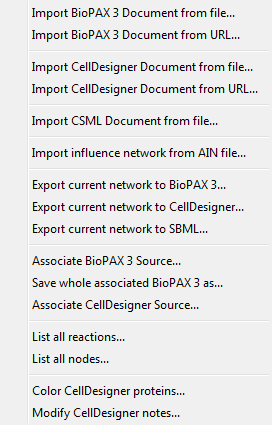
\includegraphics{graphics/BiNoM_I_O}
\end{figure}
\newpage
\section{BiNoM Analysis}
We illustrate, here, the different functions of BiNoM related to the structural analysis, using the modified version of the Novak et al. model, M-Phase.xml as an example (figure~\ref{Cytoscape_view_of_the_M-Phase_network}).
\begin{figure}
\centering
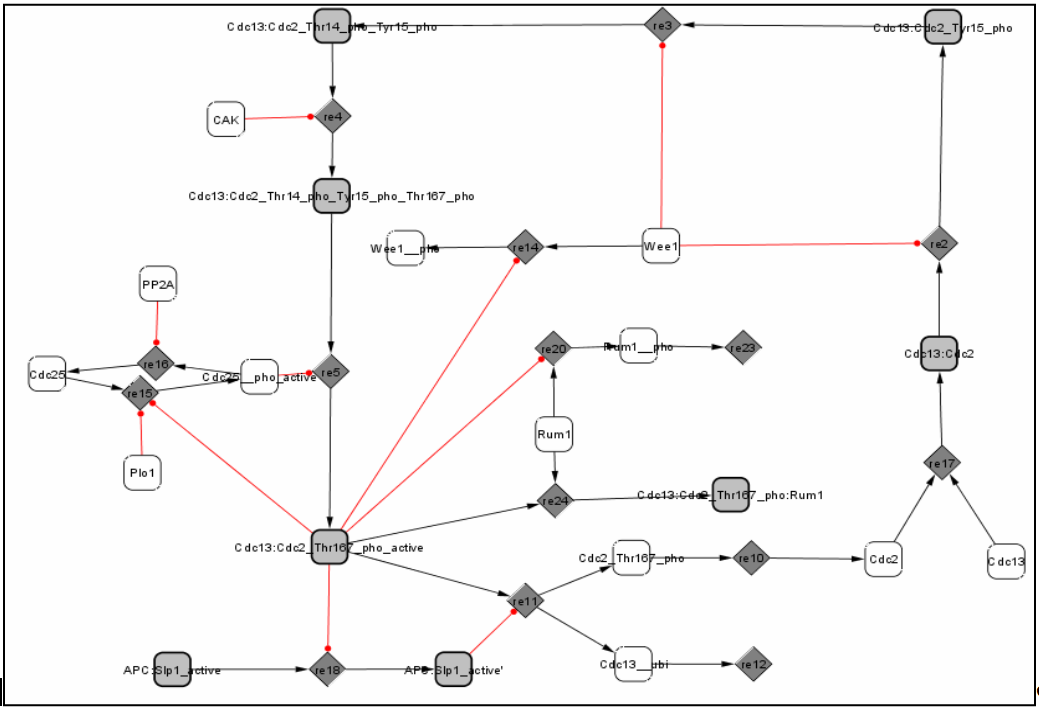
\includegraphics[width=0.8\textwidth]{graphics/Cytoscape_view_of_the_M-Phase_network.png}
\caption{Cytoscape view of the M-Phase network}
\label{Cytoscape_view_of_the_M-Phase_network}
\end{figure}
\\From the menu Plugins$\Rightarrow$BiNoM 2.1$\Rightarrow$ BiNoM analysis, we review all the functions one by one.

\subsection{Get connected components}
\textbf{Plugins$\Rightarrow$BiNoM 2.1$\Rightarrow$BiNoM Analysis$\Rightarrow$Get connected components}\\
This command dissociates the unconnected subparts of the network. In our case, since the network is already completely connected, the one obtained when choosing this function is the same as the initial one (called M-Phase.xml\_cc1).
\subsection{Get strongly connected components}
Plugins$\Rightarrow$BiNoM 2.1$\Rightarrow$BiNoM Analysis$\Rightarrow$Get strongly connected components\\
\begin{figure}
\centering
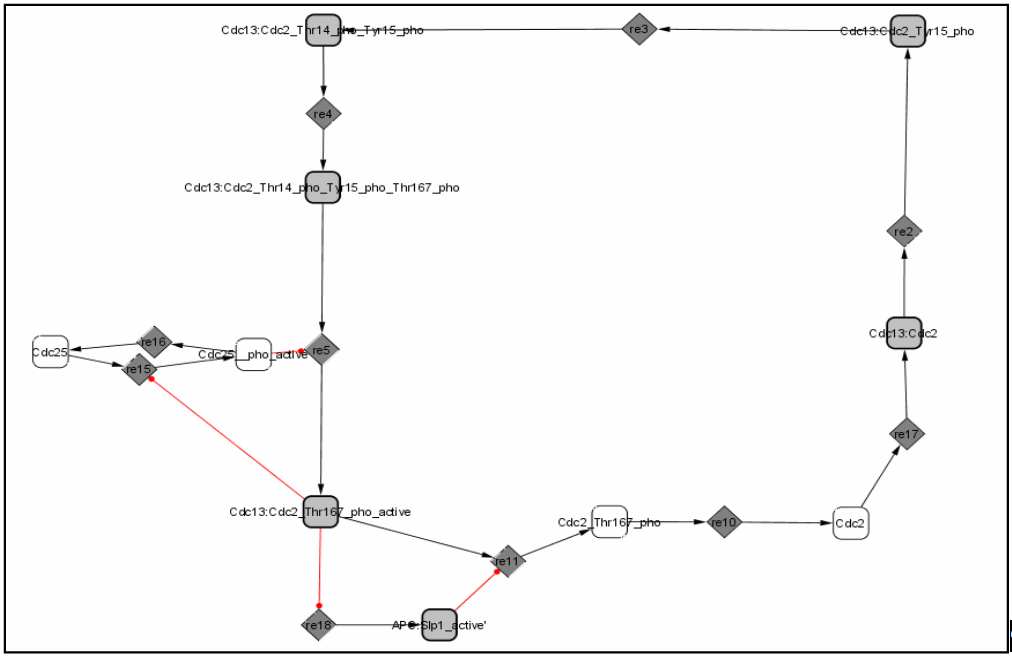
\includegraphics[width=0.8\textwidth]{graphics/Strongly_Connected_Component_of_M-Phase_network.png}
\caption{Strongly Connected Component of M-Phase network}
\label{Strongly_Connected_Component_of M-Phase_network}
\end{figure}
\\Based on Tarjan’s algorithm\cite{tarjan1972depth}, the strongly connected components are isolated. In simple words, the obtained network, M-Phase.xml\_scc1(figure~\ref{Strongly_Connected_Component_of M-Phase_network}), insures that there exists a path from one node to another and deletes the components which do not respond to this requirement.

\subsection{Prune Graph}
\textbf{Plugins$\Rightarrow$BiNoM 2.1$\Rightarrow$BiNoM Analysis$\Rightarrow$Prune graph}\\
Pruning the graph is equivalent to separating the network into three parts(figure~\ref{Prune_the_graph}: what comes in (M-Phase.xml\_in), what goes out (M-Phase.xml\_out) and the central cyclic part (M-Phase.xml\_scc).
\\This decomposition corresponds to the idea of the bow-tie structure developed by Broder and colleagues\cite{broder2000graph}. In our example, the central cyclic part is the same as figure~\ref{Strongly_Connected_Component_of M-Phase_network}, the strongly connected component. In other cases, it can be composed from several strongly connected components, connected or disconnected.\\
The Prune graph operation decomposes the current network into three parts: IN, OUT and SCC (the later can contain several strongly connected components).
\begin{figure}
\centering
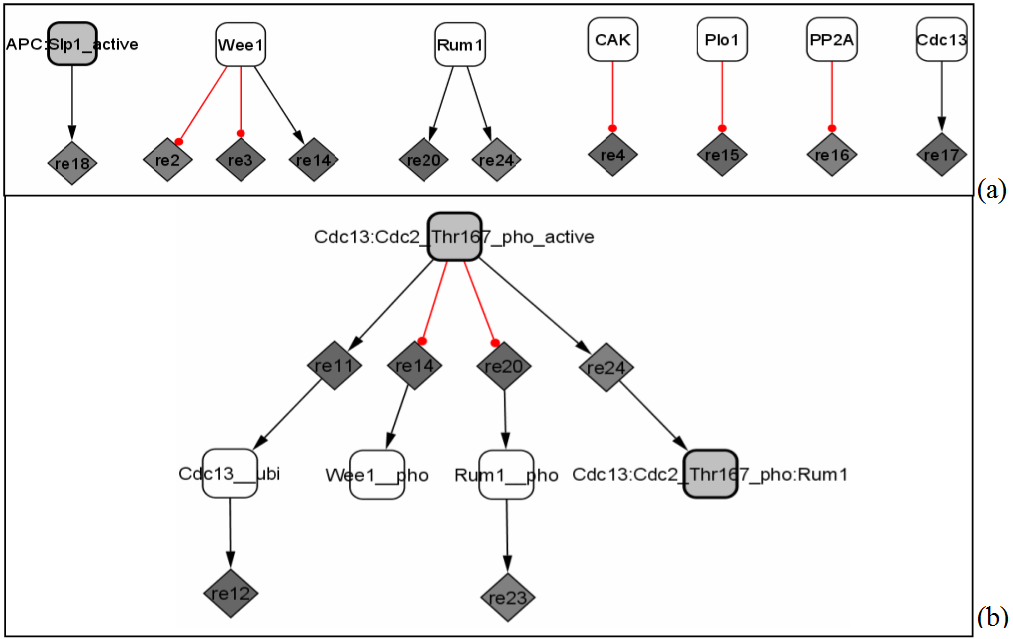
\includegraphics[width=0.8\textwidth]{graphics/Prune_the_graph}
\caption{Prune the graph. (a) Incoming flux: molecules involved in the IN part of the network, and (b) Outgoing flux: molecules involved in the OUT part of the network.}
\label{Prune_the_graph}
\end{figure}

\subsection{Get Material Components}
\textbf{Plugins$\Rightarrow$BiNoM 2.1$\Rightarrow$BiNoM Analysis$\Rightarrow$Get material components}\\
This function uses node name semantics to isolate sub-networks in which each protein takes part. In our example(figure~\ref{Material_Components}), seven sub-networks are created: M-Phase.xml\_Cdc13, M-Phase.xml\_Cdc2, M-Phase.xml\_Rum1, M-Phase.xml\_APC, M-Phase.xml\_Slp1, M-Phase.xml\_Cdc25 and M-Phase.xml\_Wee1. Some major overlaps between sub-networks are expected, as it is the case for Cdc2 and Cdc13 which form a complex.\\
\begin{figure}
\centering
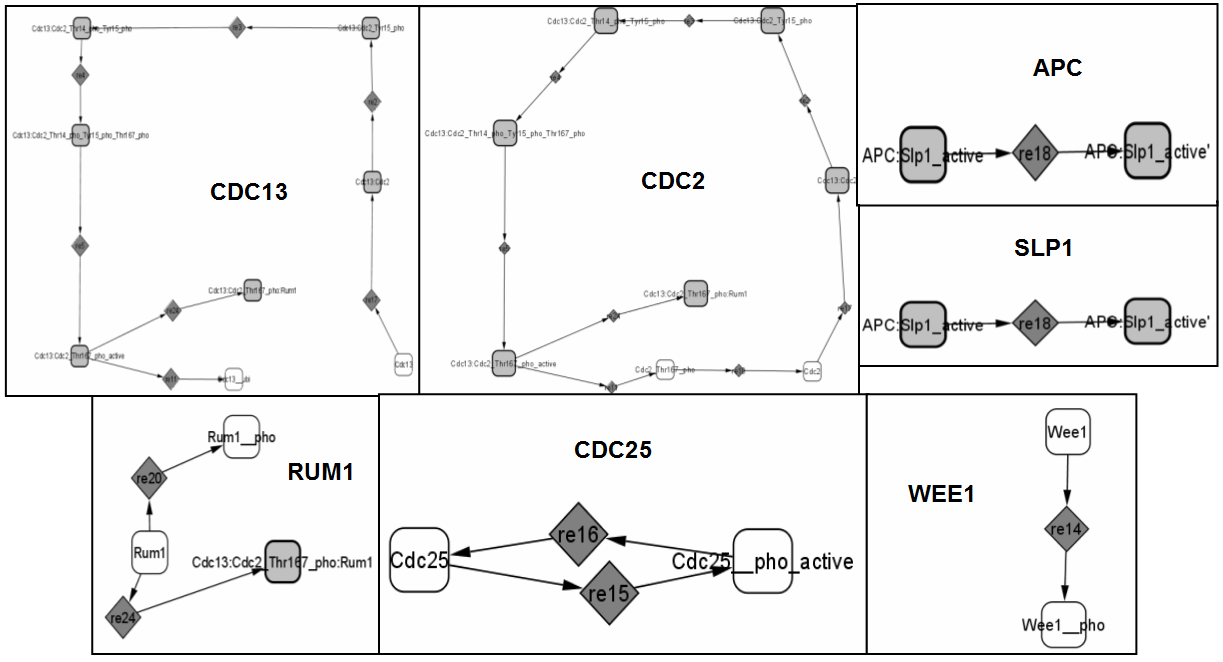
\includegraphics[width=0.8\textwidth]{graphics/Material_components}
\caption{Material Components}
\label{Material_Components}
\end{figure}

\subsection{Get Cycle Decomposition}
\textbf{Plugins$\Rightarrow$BiNoM 2.1$\Rightarrow$BiNoM Analysis$\Rightarrow$Get cycle decomposition}\\
This command decomposes the network into relevant directed cycles\cite{gleiss2001relevant}, using a modification of the Vismara’s algorithm\cite{vismara1997union}. Often, this feature gives information about the life cycle of a protein or a complex, about the feedbacks of the studied network, etc(figure~\ref{Minimal_cycle_decomposition_of_the M-Phase}). Note that the union of all the cycles corresponds to the strongly connected component figure~\ref{Strongly_Connected_Component_of M-Phase_network}.\\
\includegraphics[width=20pt,height=20pt]{graphics/warning} This operation can produce enormous number of cycles! Therefore it is rather suitable for analysis of small to moderate size networks. For a big network, one can start to understand the cyclic network structure by eliminating first the network hubs, which are contained in many network cycles. After that, the local, relatively short, cycles can be represented as meta-nodes (modules) and the analysis for cycles can be repeated.\\
\begin{figure}
\centering
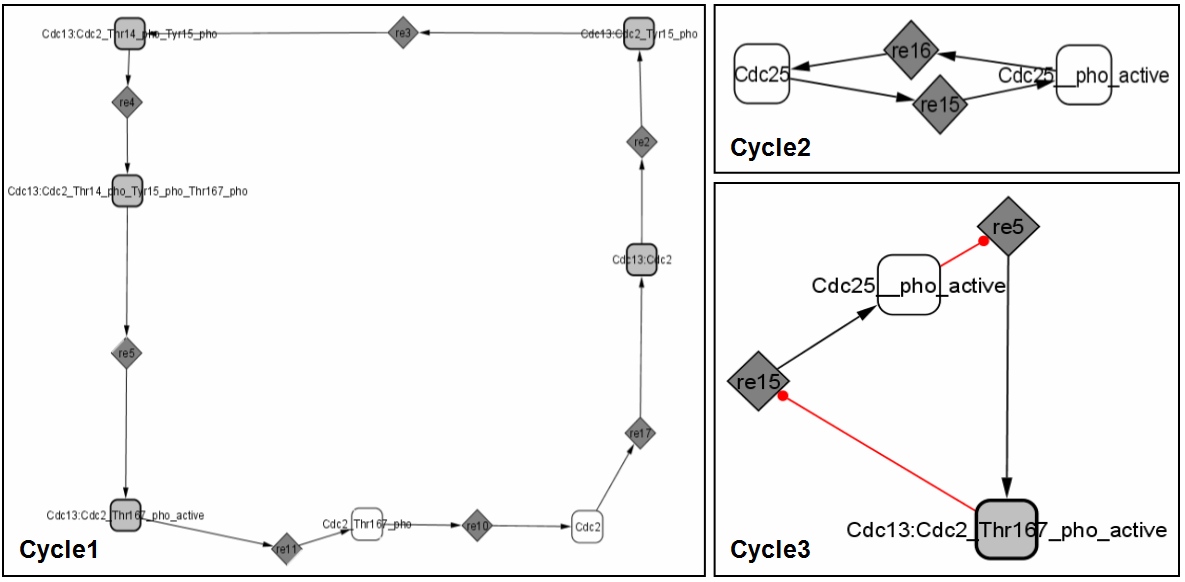
\includegraphics[width=0.8\textwidth]{graphics/Minimal_cycle_decomposition_of_the_M-Phase}
\caption{Minimal cycle decomposition of the M-Phase network.  Cycle 1 includes CDC2 and CDC13 proteins, Cycle 2 CDC25 and Cycle 3 shows the feedback existing between CDC13/CDC2 and CDC25.}
\label{Minimal_cycle_decomposition_of_the M-Phase}
\end{figure}

\subsection{Path Analysis}\label{Path_Analysis}
\textbf{Plugins$\Rightarrow$BiNoM 2.1$\Rightarrow$BiNoM Analysis$\Rightarrow$Path analysis}\\
In a network, it can become handy to find out if there exists a path (or paths) from one species to another, or to verify that a protein or a protein complex is reachable from a starting molecule(figure~\ref{Path_Analysis_All_the_paths}). Provided (an) initial source and target protein(s) that are selected first on the graph then in the dialog window, the command Path analysis can find: the shortest paths, the optimal and suboptimal shortest paths, or all the non-intersecting paths (does not include inner loops), using a finite number of intermediary nodes (use finite breadth search radius), for either directed or undirected paths (figure~\ref{Path_Analysis_Pop-up_window}).\\
\includegraphics[width=20pt,height=20pt]{graphics/warning} In big networks the number of paths can be exponential! It is recommended to find the shortest path first, take its length and increment gradually the breadth search radius starting from this value to find the second shortest, third shortest, etc., paths.\\
\begin{figure}
\centering
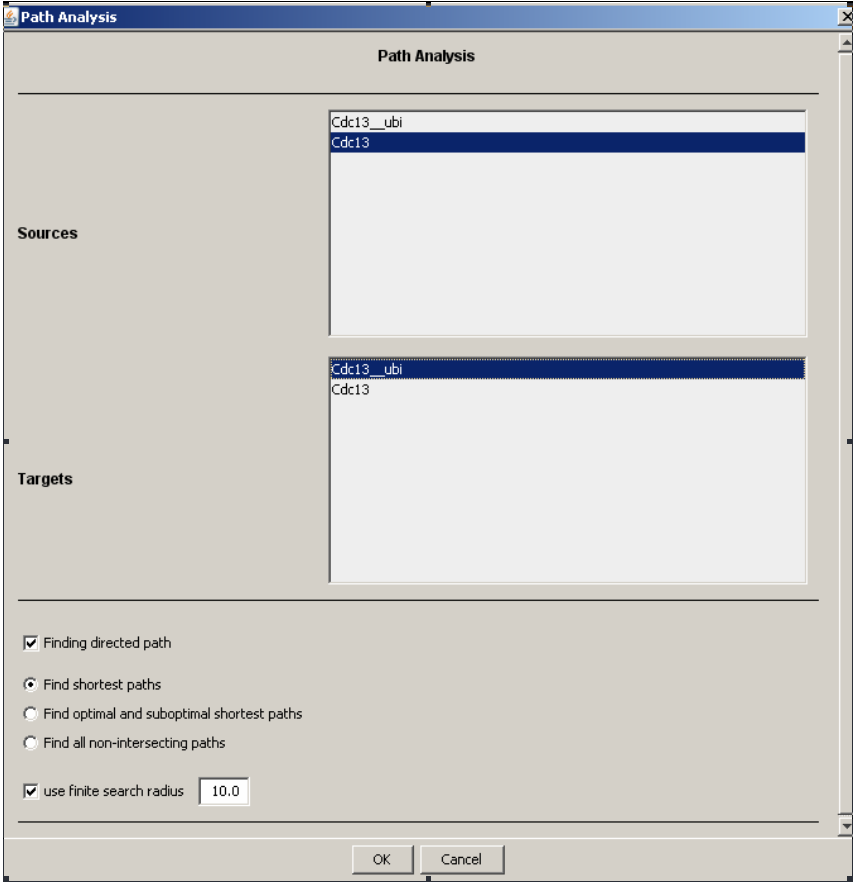
\includegraphics[width=0.8\textwidth]{graphics/Path_Analysis_Pop-up_window}
\caption{BiNoM Path Analysis: Pop-up window in which the source(s) and the target(s) need to be specified along with the type of paths (shortest, optimal shortest or all paths).}
\label{Path_Analysis_Pop-up_window}
\end{figure}
\begin{figure}
\centering
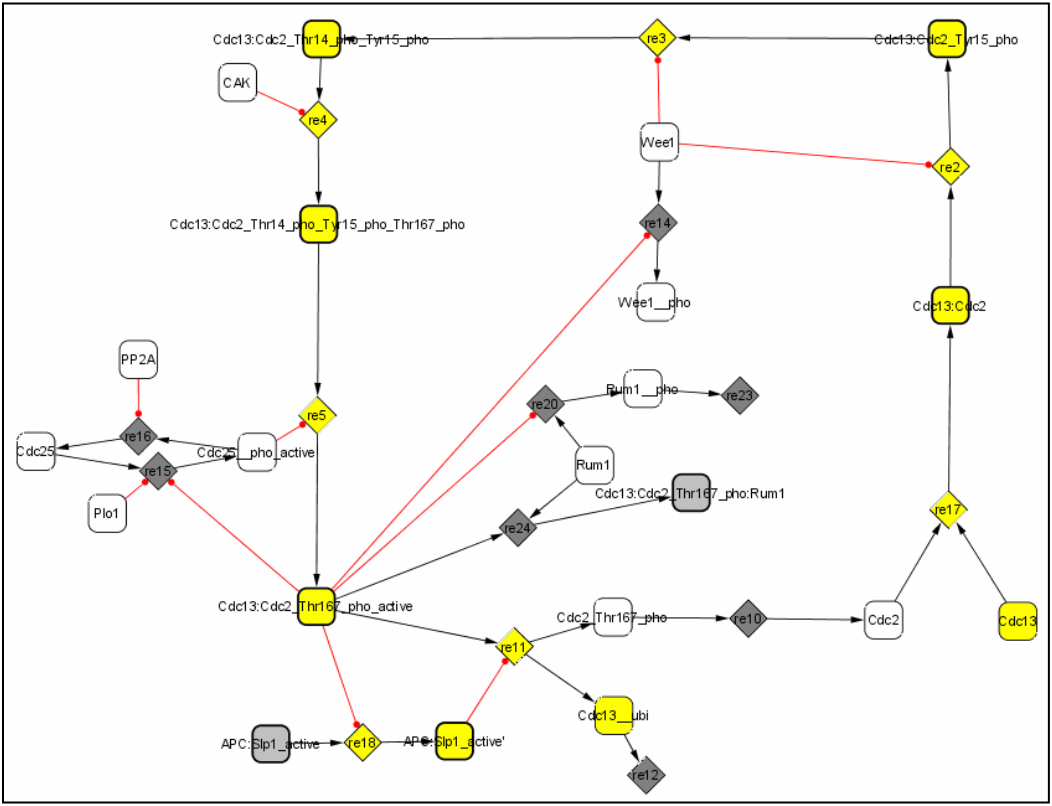
\includegraphics[width=0.8\textwidth]{graphics/Path_Analysis_All_the_paths}
\caption{Path Analysis: All the paths leading from one molecular species (Cdc13) to another (Cdc13\_ubi, ubiquitinated form of Cdc13) are highlighted in yellow.}
\label{Path_Analysis_All_the_paths}
\end{figure}

\subsection{Extract subnetwork}
\textbf{Plugins$\Rightarrow$BiNoM 2.1$\Rightarrow$BiNoM Analysis$\Rightarrow$Extract subnetwork}\\
Extract a subnetwork from selected nodes of a network with various options (figure~\ref{Extract_subnetwork_dialog}).
\begin{figure}
\centering
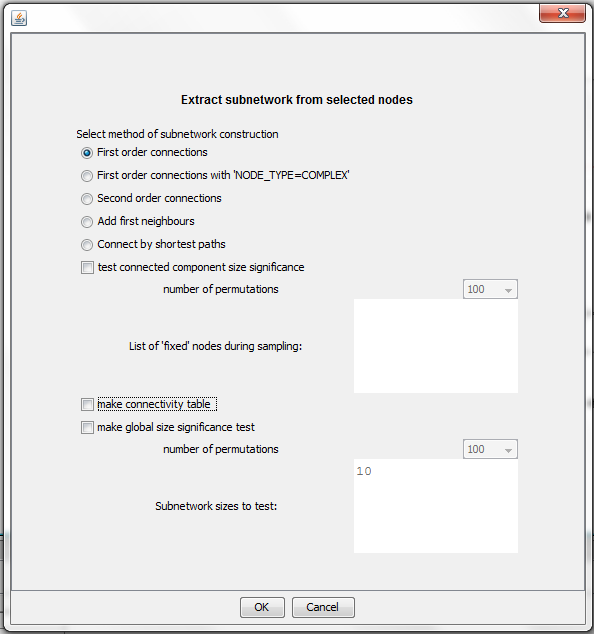
\includegraphics[width=0.8\textwidth]{graphics/Extract_subnetwork_dialog}
\caption{Dialog of the ``Extract subnetwork'' function showing the different options available.}
\label{Extract_subnetwork_dialog}
\end{figure}

\subsection{Calc centrality, Inbetweenness undirected, Inbetweenness directed}
\textbf{Plugins$\Rightarrow$BiNoM 2.1$\Rightarrow$BiNoM Analysis$\Rightarrow$Calc centrality$\Rightarrow$Inbetweenness undirected}
\textbf{Plugins$\Rightarrow$BiNoM 2.1$\Rightarrow$BiNoM Analysis$\Rightarrow$Calc centrality$\Rightarrow$Inbetweenness directed}
Display centrality of nodes in cases undirected and directed.

%\subsection{Generate Modular View}
%\textbf{Plugins$\Rightarrow$BiNoM$\Rightarrow$analysis$\Rightarrow$Generate modular view}\\
%Given the initial diagram and some modules (which could be sub-networks of the initial network), it is possible to reconstruct a modular view of the network. For our example, we choose the initial network to be M-Phase.xml and the subparts or modules, the seven sub-networks corresponding to the material components described in (4). From these seven sub-networks only six are selected since two of them, Slp1 and APC, are exactly the same.\\
%The sub-networks or modules need to be specified in the “creating modular view” window (figure~\ref{Modular_view_Pop-up_window}).\\
%\begin{figure}
%\centering
%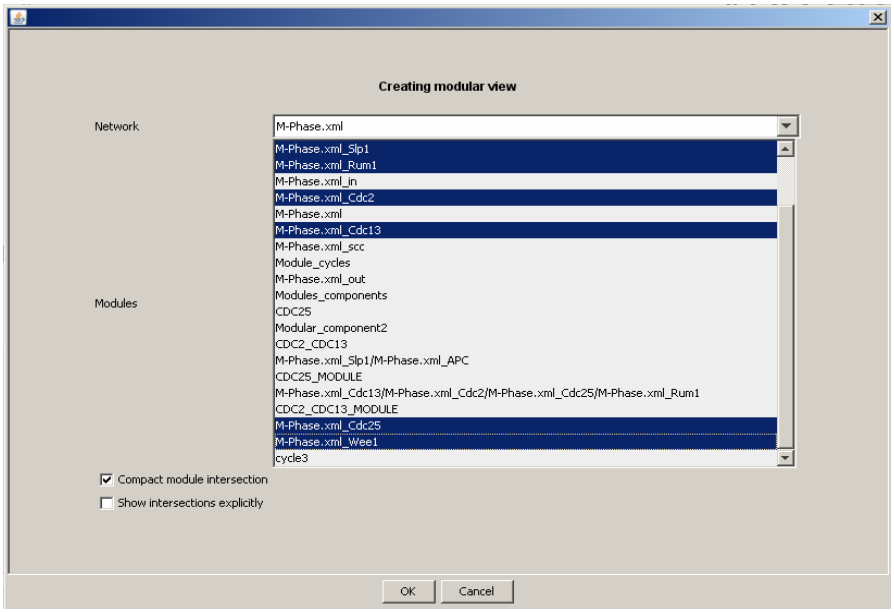
\includegraphics[width=0.8\textwidth]{graphics/Modular_view_Pop-up_window}
%\caption{BiNoM modular view of the newtork: Pop-up window in which the initial graph and the modules are specified. }
%\label{Modular_view_Pop-up_window}
%\end{figure}
%\\There are different types of modular views. The modules are connected by: (1) the number of shared interactions (figure~\ref{Modular_view_The_resulting_modular_network}, upper panel); (2) the number of shared nodes (reactions + species) for which case the box “Compact module intersection” must be checked (figure~\ref{Modular_view_The_resulting_modular_network}, middle panel); and (3) the shared nodes and reactions showed explicitly (figure~\ref{Modular_view_The_resulting_modular_network}, lower panel).
%\begin{figure}
%\centering
%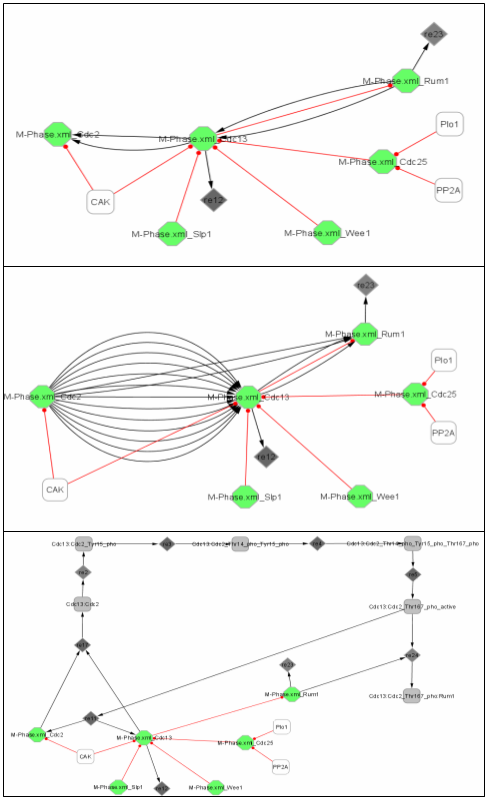
\includegraphics[width=0.8\textwidth]{graphics/Modular_view_The_resulting_modular_network}
%\caption{BiNoM modular view of the newtork: The resulting modular network (upper panel) with compact module intersections (middle panel) and with explicit intersections (lower panel).}
%\label{Modular_view_The_resulting_modular_network}
%\end{figure}

\subsection{Cluster Networks}
\textbf{Plugins$\Rightarrow$BiNoM 2.1$\Rightarrow$BiNoM Analysis$\Rightarrow$Cluster networks}\\
This command lumps together the modules that share a certain proportion of nodes. At a first glance, it can easily be concluded from Figure~\ref{Modular_view_The_resulting_modular_network} (middle panel) that, for example, the modules M-Phase.xml\_Cdc13 and M-Phase.xml\_Cdc2 share a lot of proteins or protein complexes. Therefore, we can assume that these two modules will collapse into one big module. To determine the clusters, the intersection threshold can be set (from 0 to 100\% intersecting components). For a 30\% intersection threshold, Figure~\ref{Clusters_of_modules_using_the_material_decomposition} is obtained. Four clusters of modules were proposed and linked.\\\\
An alternative modular view has been obtained using the cycle decomposition instead of the material decomposition. The cycles are presented in Figure~\ref{Minimal_cycle_decomposition_of_the M-Phase}. They are obtained by clustering the three cycles into two (cycle 1 + cycle2/cycle3) and organized into a modular view (Figure~\ref{Clusters_of_modules_using_the_cycle_decomposition}).\\
\begin{figure}
\centering
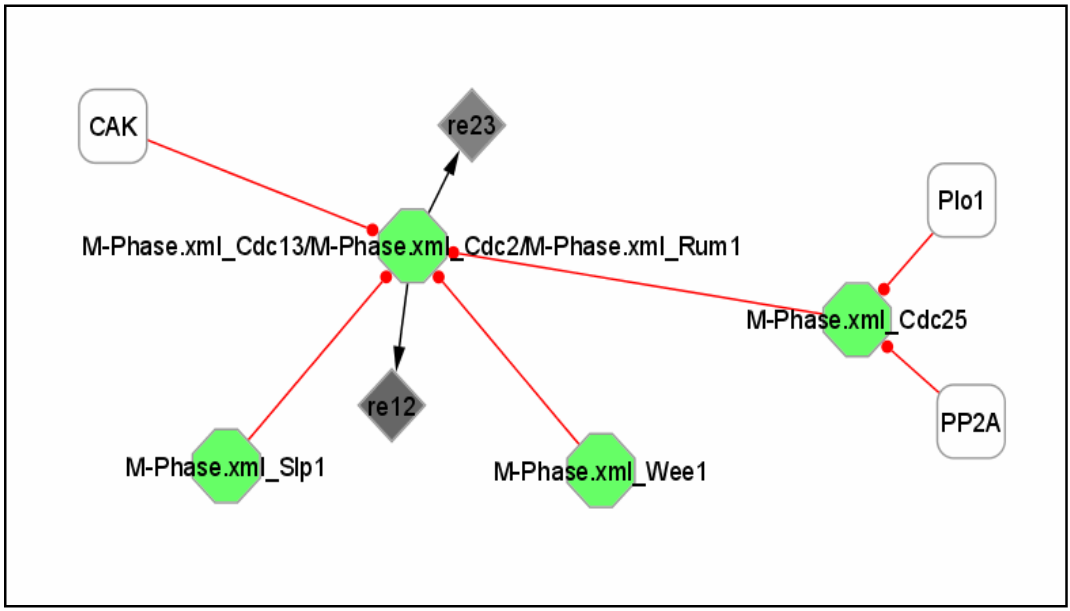
\includegraphics[width=0.8\textwidth]{graphics/Clusters_of_modules_using_the_material_decomposition}
\caption{Clusters of modules. The obtained diagram is a compact modular view of the M-Phase network using the material decomposition and material components clustering}
\label{Clusters_of_modules_using_the_material_decomposition}
\end{figure}
\begin{figure}
\centering
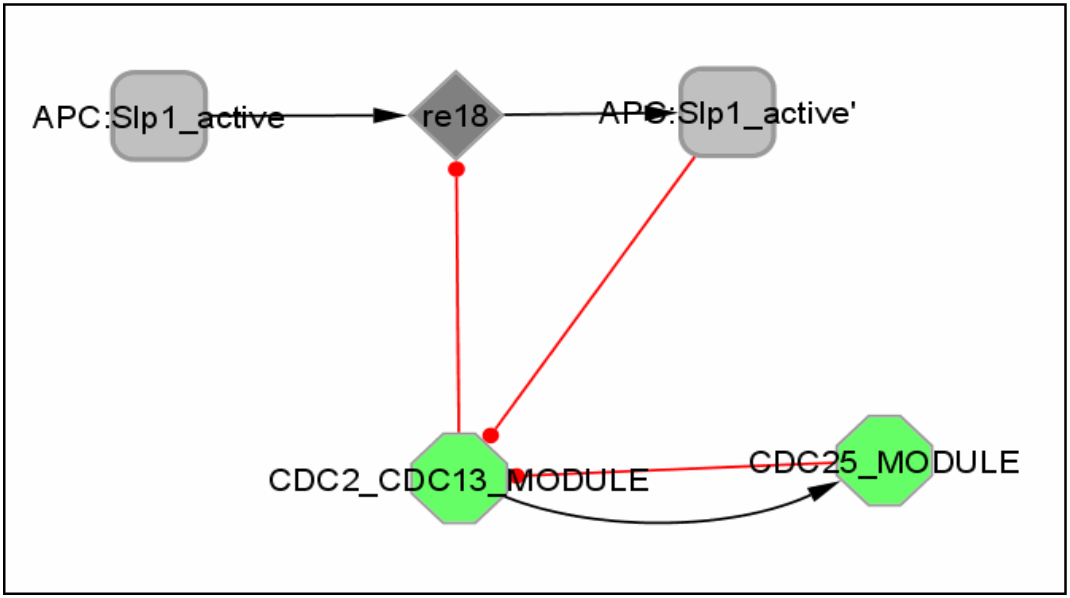
\includegraphics[width=0.8\textwidth]{graphics/Clusters_of_modules_using_the_cycle_decomposition}
\caption{Clusters of modules. The obtained diagram is a compact modular view of the M-Phase network using the relevant cycle decomposition and cycle clustering}
\label{Clusters_of_modules_using_the_cycle_decomposition}
\end{figure}

\subsection{Mono-molecular react.to edges}
\textbf{Plugins$\Rightarrow$BiNoM 2.1$\Rightarrow$BiNoM Analysis$\Rightarrow$Mono-molecular react. to edges}\\
This function transforms monomolecular reaction nodes (i.e. reactions with one
reactant and one product) into ‘influence’ edges. Thus, monomolecular (linear)
reactions are represented as edges and the reaction graph is not bi-partite
anymore. When the reaction nodes have the type of influence specified (through
the Cytoscape ‘EFFECT’ attribute), the graph is transformed automatically into an
influence graph (see Figure~\ref{Network_to_influence_graph}: upper panel:
BioPAX network, lower panel, the equivalent influence network). Non-linear
non-monomolecular reactions (such as complex assemblies) are not transformed and
remain to be represented as network nodes.
\begin{figure}
\centering
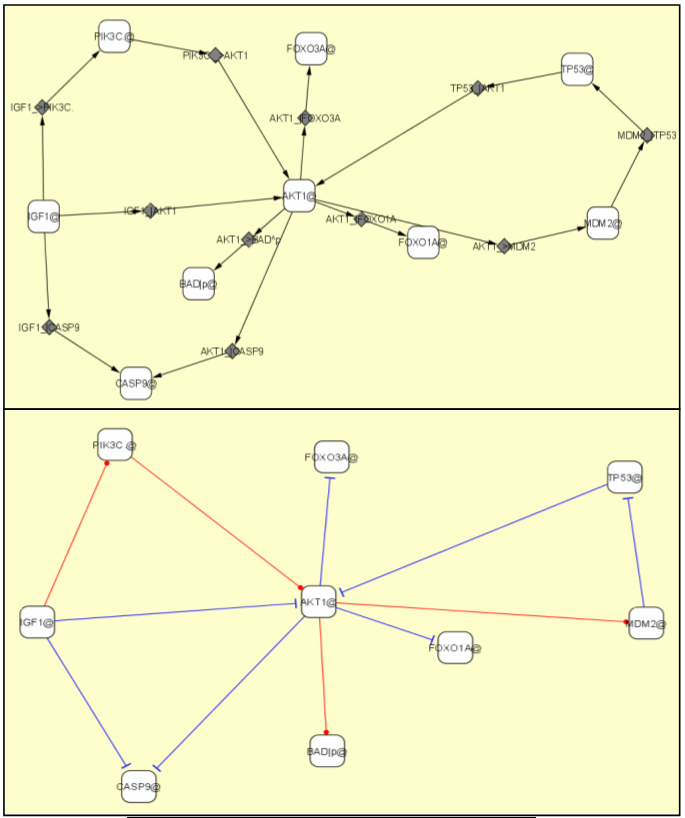
\includegraphics[width=0.8\textwidth]{graphics/Network_to_influence_graph}
\caption{From a BioPAX network (upper panel) to an influence graph (lower panel).}
\label{Network_to_influence_graph}
\end{figure}

\subsection{Linearize network}

%Remove reactions and reconnect edges according to a supposed influence (figure~\ref{Linearized_Network_M-Phase})\\
%\includegraphics[width=20pt,height=20pt]{graphics/warning} The got network is not an influence network in the biological sense. But, it can be used to build an influence network.
%\begin{figure}
%\centering
%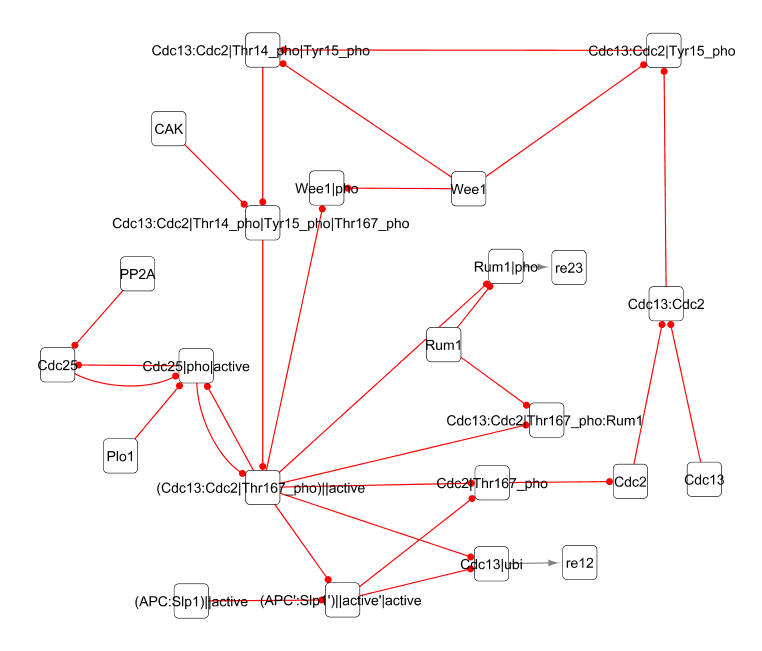
\includegraphics[width=0.8\textwidth]{graphics/Linearized_Network_M-Phase}
%\caption{Result of applying "Linearize network" to M-Phase.}
%\label{Linearized_Network_M-Phase}
%\end{figure}
The ``linearization'' replaces explicit reactions of complex formation by direct influences between constituents and complexes (in the case of an influence network imported from an AIN file).

To illustrate this function, import the AIN file \textit{cell\_cycle\_AIN.txt}.

\textbf{Plugins$\Rightarrow$BiNoM 2.1$\Rightarrow$BiNoM I/O$\Rightarrow$Import influence network from AIN file...}\\
Click two times 'OK' for the specification of the families. A new network is created. Then, apply the linearization functions
\textbf{Plugins$\Rightarrow$BiNoM 2.1$\Rightarrow$BiNoM Analysis$\Rightarrow$‘Linearize’ network}\\

A new 'linearized' network is created (figure ~\ref{Linearized_Network_Cell_Cycle}).

\begin{figure}
  \centering
  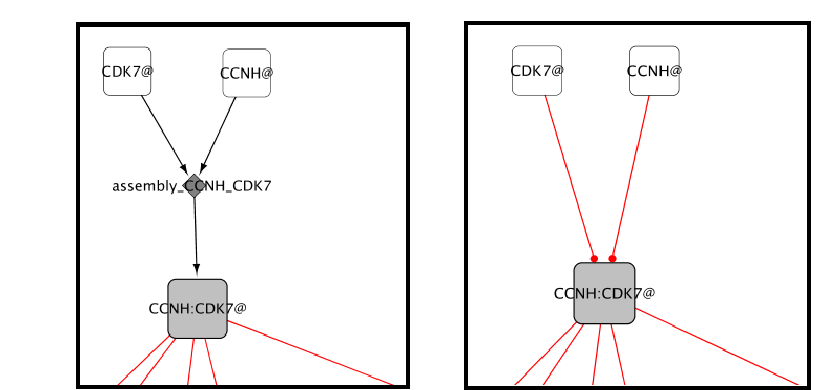
\includegraphics[width=0.8\textwidth]{graphics/linearize_cc.pdf}
  \caption{Example of explicit reaction of complex formation (left panel) that can be replaced by direct connections (right panel) using the ``linearization`` function of BiNoM.}
  \label{Linearized_Network_Cell_Cycle}
\end{figure}


\subsection{Exclude intermediate nodes}
\textbf{Plugins$\Rightarrow$BiNoM 2.1$\Rightarrow$BiNoM Analysis$\Rightarrow$Exclude intermediate nodes}\\
This function opens a dialog where nodes to be excuded can be selected (figure~\ref{Exclude_nodes_Dialog}). It creates a network without the selected nodes and reconnects edges.
\begin{figure}
\centering
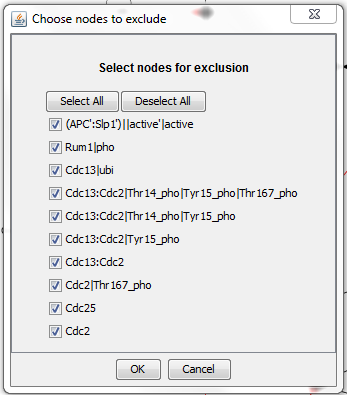
\includegraphics[width=7 cm]{graphics/Exclude_nodes_Dialog}
\caption{Dialog to select nodes to be excluded in the created network.}
\label{Exclude_nodes_Dialog}
\end{figure}

\subsection{Extract Reaction Network}
\textbf{Plugins$\Rightarrow$BiNoM 2.1$\Rightarrow$BiNoM Analysis$\Rightarrow$Extract reaction networks}\\
This function cleans up the diagram to only keep the reaction network. Only nodes with ‘XXXX\_REACTION’ and ‘XXXX\_SPECIES’ attributes (where XXXX stands for any word) are kept as a result of this operation. For example, it helps to clean the reaction network interface from the result of querying BioPAX index (which contains many other node types such as entities and publications.

\subsection{Path Influence Quantification analysis}
\textbf{Plugins$\Rightarrow$BiNoM 2.1$\Rightarrow$BiNoM Analysis$\Rightarrow$Path Influence Quantification analysis}\\

%This function is based on an algorithm of  Path Influence Quantification
%(PIQuant). Shortly, for every annotated nodes, the influence is computed by
%summing (optimal and sub-optimal) paths contribution (1/(length of the path)),
%multiplied by the nodes annotation that represent biological data. For global
%influence computation, influences are summed on all over the annotated nodes.
%The figure \ref{PIQuant_example} shows the computing in a simple example.\\\\

This function calculates a score to quantify the effect of experimental data
onto one or more target nodes for a given network architecture, named the
PIQuant score (Pathway Influence Quantification). The target node can be a gene
or a phenotype of interest (such as cell cycle or apoptosis). We define as
annotated nodes any node of the network for which we have experimental data
available. The experimental data can be for instance an mRNA expression value
(ratio disease/normal). We also assume that we have determined all the paths
from the annotated nodes to the target nodes using an appropriate algorithm
(such as Dijkstra's shortest paths algorithm). The PIQuant score is then defined as:


$$
 PIQuant_{Score} = \sum_{k=1}^{q} \alpha_{k} \sigma_{k} \frac{1}{\lambda_{k}}
$$

 A path $k \in \{1,\ldots , q\}$ is defined
as a the sequence of consecutive connected nodes
between a source node and a target node (without repetition of any node
or edge).

The annotation $\alpha_k$ of the path $k$ is defined as the annotation (real value representing the experimental data) 
of its source node. We define the sign $\sigma_k$
of the path $k$ as the product of the signs of every edge of the path and finally
the length $\lambda_k$ of the path $k$ as the number of edges in the path. We
hypothesize that the longer the path is, the lesser the global influence will be
on the target node.

\includegraphics[width=20pt,height=20pt]{graphics/warning} The Cytoscape edge attribute
which encodes the influence corresponding to the sign (+1 or -1) of the edge is "EFFECT" which can take 2 values EFFECT:activation and
EFFECT:inhibition.\\\\

\begin{figure}
  \centering
  %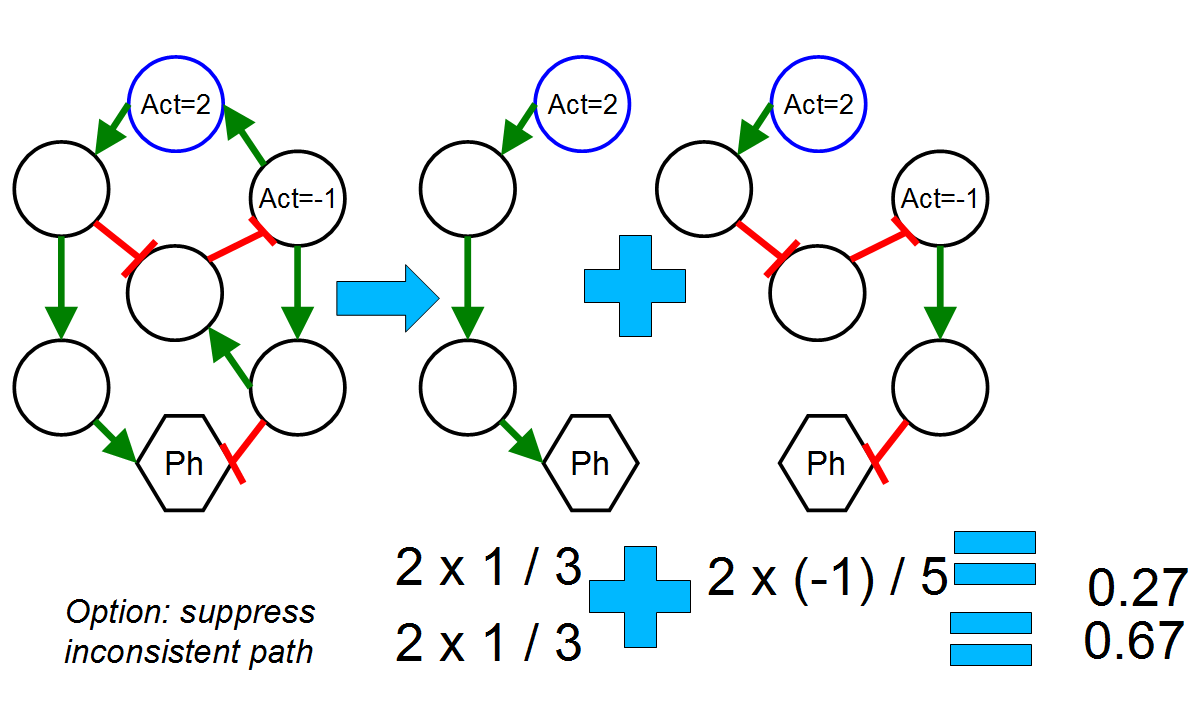
\includegraphics[width=0.8\textwidth]{graphics/PIQuant_example}
  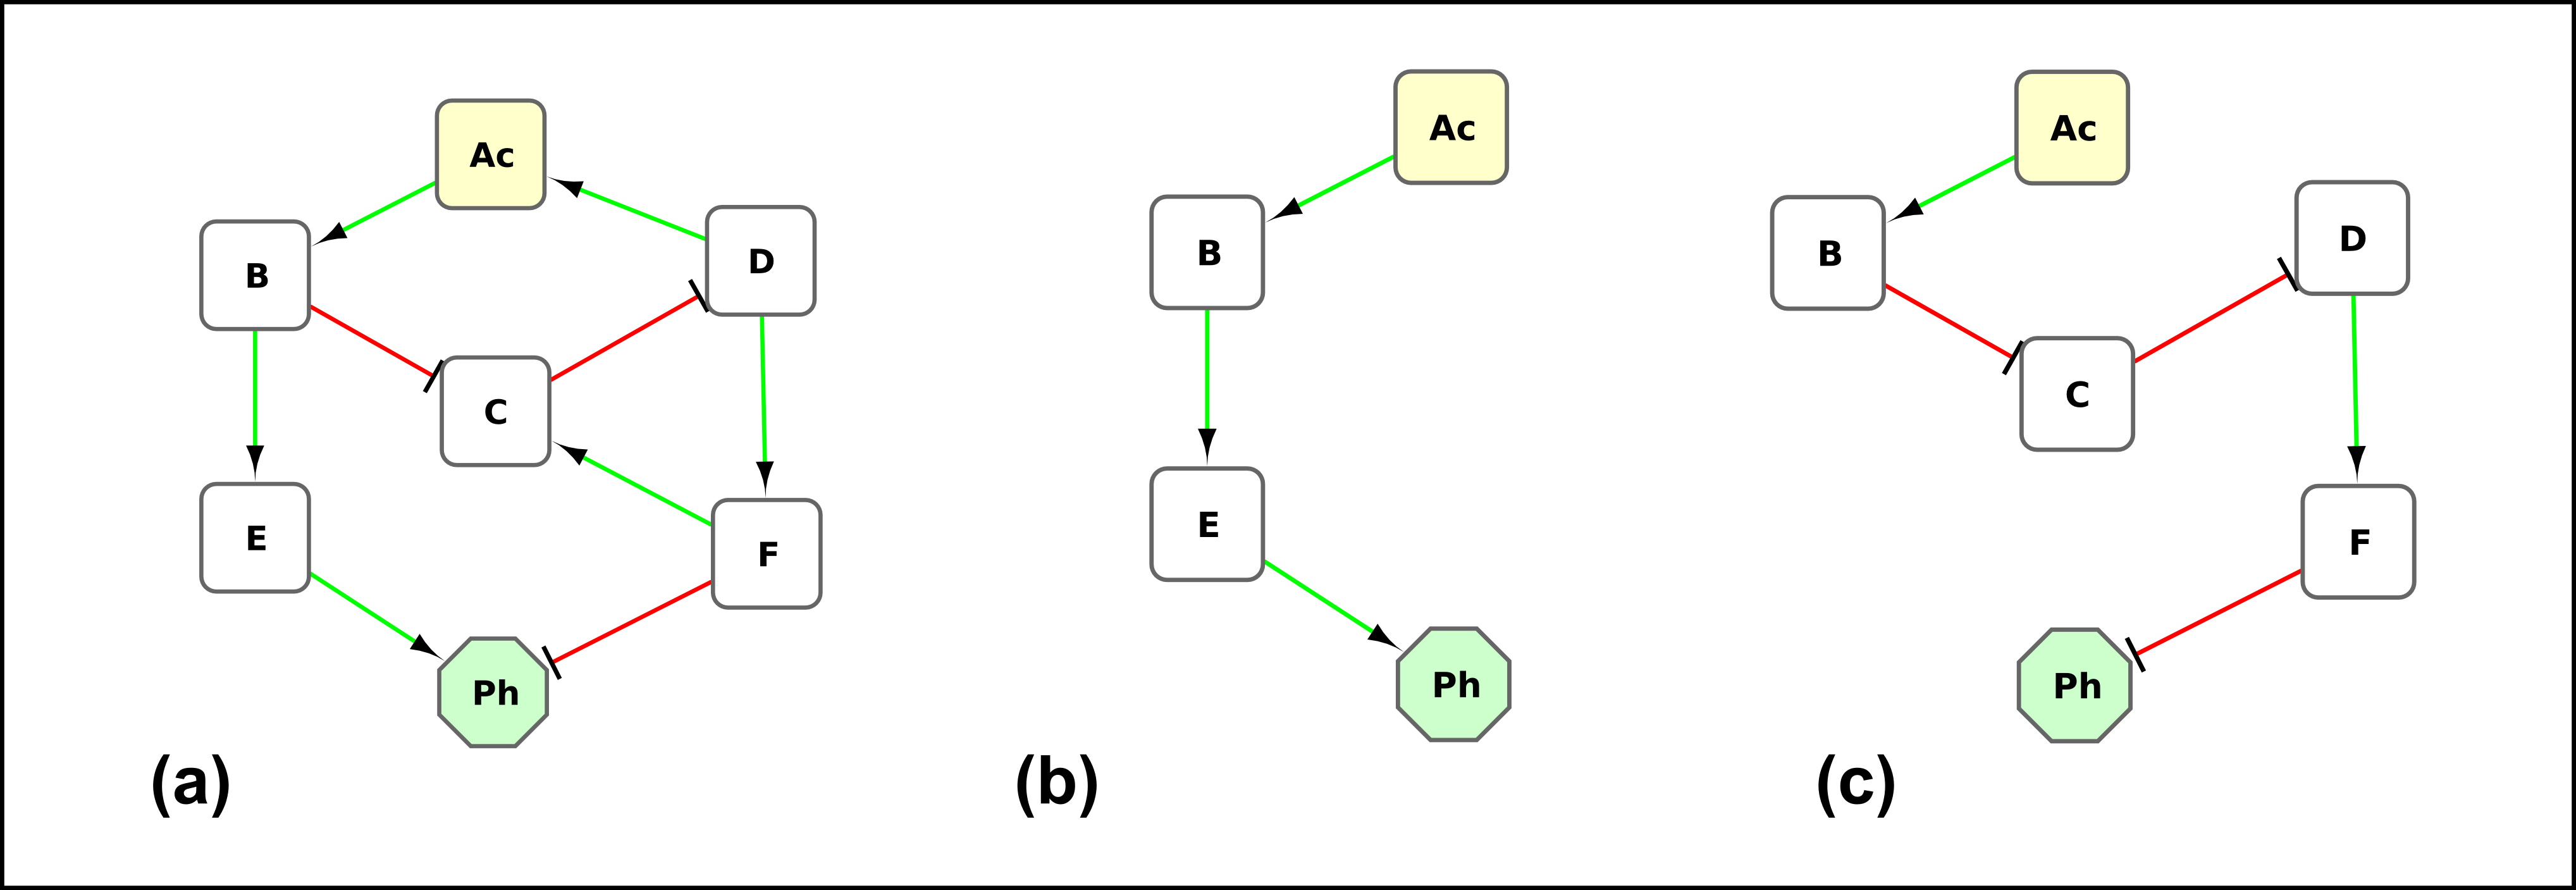
\includegraphics[width=0.8\textwidth]{graphics/piquant_networks}
  \caption{A simple influence network. The network is composed of seven nodes
and nine edges (a). The two paths (b,c) extracted from this network start from
the source node \textbf{Ac} and end at the target node \textbf{Ph} (a phenotype of interest). The
nodes \textbf{Ac} and \textbf{D} are annotated using experimental data, and have the values 2.0
and -1.0 respectively.}
  \label{PIQuant_example}
\end{figure}


In the case of the network presented in figure~\ref{PIQuant_example}a, let us
consider Ac the source node and Ph the target node and consider only the two
paths defined in the figure~\ref{PIQuant_example}b and
figure~\ref{PIQuant_example}c. Given that the
node Ac is annotated by the value $2.0$, that the first path has a length
equal to 3, and that the second path has a length equal to 5, we can calculate the PIQuant score
of the node Ac to the node Ph as:

$$
 PIQuant_{Score} = 2 \cdot 1 \cdot \frac{1}{3} + 2 \cdot (-1) \cdot \frac{1}{5}
= 0.27
$$


Sometimes a path has one or more intermediate nodes that are annotated nodes
(i.e. for which we have experimental data values),
in addition to the source node.
In that case, the intermediate node is \textit{consistent} if the sign of its
annotation is the same as the sign of the source node annotation multiplied by
the sign of the
path from the source node to the intermediate node. If signs are opposite, the
node is \textit{inconsistent}.
A path is \textit{consistent} if each annotated intermediate nodes is
consistent. A path is \textit{inconsistent} if at least one intermediate node is
\textit{inconsistent}.
In other words, a path is inconsistent when the
sign of the experimental data value for a node is opposite to the sign
of the path.

For example, according to the network represented in figure~\ref{PIQuant_example}c, there is an influence from Ac to Ph
that goes through D . But if this path
is functional, the annotation of node D should have the same sign as the annotation for node Ac, because
Ac activates D indirectly (i.e. the path from Ac to D has a positive sign). In this case, the sign of D annotation (the experimental value) is opposite to
the sign of Ac annotation, and therefore, the path from Ac to Ph that goes through D is inconsistent.

Practically, we offer the option to
keep or not the inconsistent paths for the calculation of the PIQuant score,
depending on how the user wants to analyze the calculations. An inconsistent
path could indicate that the path is not complete, or could also indicate that
the path is correct but not active under the precise conditions in which the
experimental data was generated, corresponding to a different context.

In the case mentionned above in figure~\ref{PIQuant_example}c, if only consistent paths are kept, then the PIQuant score of Ac to Ph
becomes:

$$
 PIQuant_{Score} = 2 \cdot 1 \cdot \frac{1}{3} = 0.67
$$

This score is higher than the value previously obtained with all the paths, and can be interpreted in this case as a higher activation of the phenotype.


In order to calculate the PIQuant score, an influence network with annotated
nodes should be created, for example using the AIN file format (see the AIN file
format description in the appendix).

One the network is created in Cytoscape, then we can call the BiNoM function to calculate the PIQuant score.

\textbf{Plugins$\Rightarrow$BiNoM 2.1$\Rightarrow$BiNoM Analysis$\Rightarrow$Path Influence Quantification analysis}\\

%For global influences, a p-value can be computed, by shuffling the annotation.
%Among the possible options accessible in BiNoM, the possibility of removing
%inconsistent path (paths that have an intermediate node with inconsistent
%annotation) was sometimes used.\\\\

This function has two dialogs, one for choosing the annotated nodes, targets nodes and path search algorithm, and one to display the results of the calculation.

Step 1 see figure~\ref{Path_consistency_analyser_Dialog1}:

\begin{itemize}
  \item Select the attribute name corresponding to the annotation and click update list, only active nodes are
  displayed in box.
  \item Select target nodes.
  \item Choose one algorithm for path searching, see glossary in section \ref{GLOSSARY} for details on the different algorithms.
  \item Click OK.
\end{itemize}

\begin{figure}
  \centering
  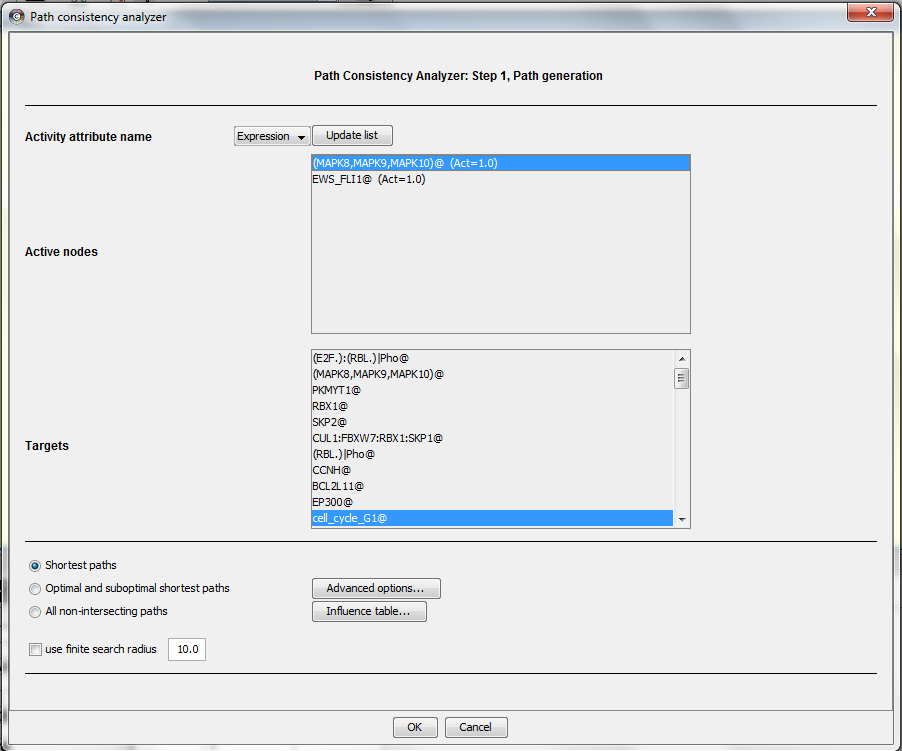
\includegraphics[width=0.8\textwidth]{graphics/Path_consistency_analyser_Dialog1}
  \caption{Path consistency analysis: dialog of step 1, select annotated nodes,
targets and the algorithm for searching the paths.}
  \label{Path_consistency_analyser_Dialog1}
\end{figure}

The step 2 dialog (the results of the PIQuant score calculations) is displayed on figure~\ref{Path_consistency_analyser_Dialog2}.



\begin{figure}
  \centering
  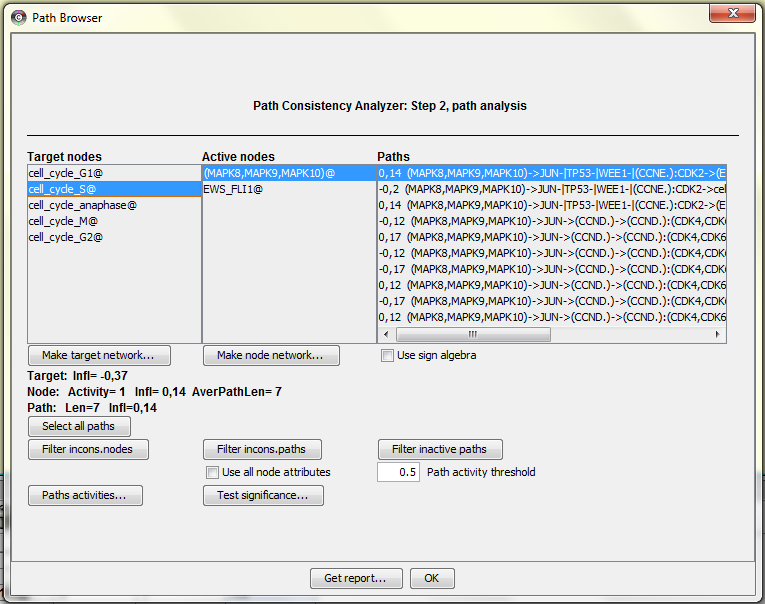
\includegraphics[width=0.8\textwidth]{graphics/Path_consistency_analyser_Dialog2}
  \caption{Path consistency analysis: dialog of step 2, display paths and
activities, get all results}
  \label{Path_consistency_analyser_Dialog2}
\end{figure}  

%\subsection{OCSANA analysis}
%\textbf{Plugins$\Rightarrow$BiNoM 2.1$\Rightarrow$BiNoM Analysis$\Rightarrow$OCSANA analysis}\\
%Work in progress.

\subsection{Create neighborhood sets file}
\textbf{Plugins$\Rightarrow$BiNoM 2.1$\Rightarrow$BiNoM Analysis$\Rightarrow$Create neighborhood sets file}\\
This function creates a file *.gmt (a text file where nodes are separated by \textless Tab\textgreater) containing the neighbors of selected nodes according to option of the dialog(figure~\ref{Create_Neigborhood_File_Dialog})
\begin{figure}
\centering
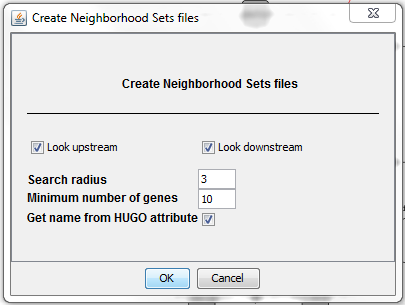
\includegraphics[width=7 cm]{graphics/Create_Neigborhood_File_Dialog}
\caption{Diialog for options of creating a neighborhood sets file.}
\label{Create_Neigborhood_File_Dialog}
\end{figure}  

\newpage
\section{BiNoM Module Manager}
Module manager is useful for creating modular view of large networks without loosing details of modules (using “nest”, object of Cytoscape v7 and after).

\subsection{Create Network of Modules}
\textbf{Plugins$\Rightarrow$BiNoM 2.1$\Rightarrow$BiNoM Module Manager$\Rightarrow$Create Network of Modules}\\
Create a new network from a list of sub-networks (sub-networks are selected in the network list see figure~\ref{Create_network_of_modules}).\\
Nodes=modules, no edge. Visual style created in VizMapper for module network . The got network is as \ref{M-Phase_Material_Modular} without edge and with nodes on grid.\\
\includegraphics[width=20pt,height=20pt]{graphics/warning} Module names and node names must be different, all network names too.\\\\
To go from module to sub-network:\\
select node$\Rightarrow$CRight click$\Rightarrow$CNested Network$\Rightarrow$Go to Nested Network.
\begin{figure}
\centering
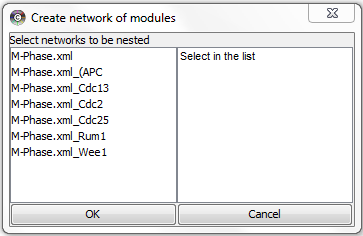
\includegraphics[width=0.8\textwidth]{graphics/Create_network_of_modules}
\caption{Dialog for select networks to become modules in modular0}
\label{Create_network_of_modules}
\end{figure}

\subsection{Create Connections between Modules}
\textbf{Plugins$\Rightarrow$BiNoM 2.1$\Rightarrow$BiNoM Module Manager$\Rightarrow$Create Connections between Modules}\\
Create edges linking modules from all edges of the selected network.\\
Links are simplified, no distinction between left and right (molecule flow), no duplication if same interaction.\\
Warning message if duplicated or absent nodes (may disturb links).
\begin{figure}
\centering
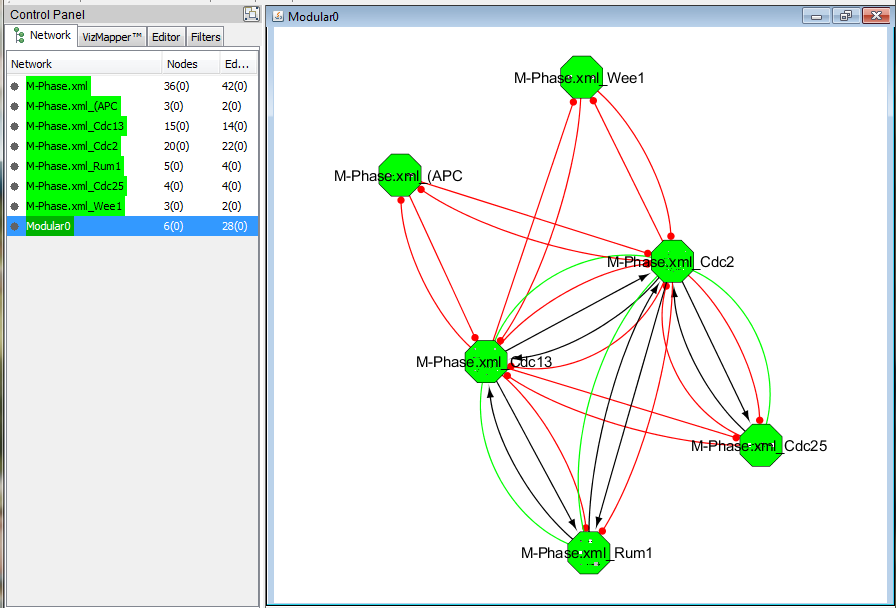
\includegraphics[width=0.8\textwidth]{graphics/M-Phase_Material_Modular}
\caption{M-Phase is divided into modules by get material component. The modular view is got by creating network of modules with organic layout. The function "Create connections between modules" links modules according to the reference network. The function "Find common nodes in modules" creates intersection edges. }
\label{M-Phase_Material_Modular}
\end{figure}

\subsection{Create Modules from Networks}
\textbf{Plugins$\Rightarrow$BiNoM 2.1$\Rightarrow$BiNoM Module Manager$\Rightarrow$Create Modules from Networks}\\
Create modules in the active network from a list of sub-networks (sub-networks are selected in the network list)\\
All edges are kept. See edge attribute PREVIOUS\_ID for their origin.\\
The attribute BIOPAX\_NODE\_TYPE is set to “pathway” (see visual style BiNoM BioPAX).\\
\includegraphics[width=20pt,height=20pt]{graphics/warning} All nodes of sub-networks must be found once in the active network (no intersection between sub-networks).

\subsection{Agglomerate the Nearest Nodes in Modules}
\textbf{Plugins$\Rightarrow$BiNoM 2.1$\Rightarrow$BiNoM Module Manager$\Rightarrow$Agglomerate the Nearest Nodes in Modules}\\
Create modules and a modular view by agglomerating the nearest nodes in the active network (see~algorithm~in section~\ref{Agglomeration_by_shortest_path}.\\\\
Input 2 parameters to get not too big sub-networks containing not too far nodes:
\begin{itemize}
\item Maximal distance between nodes or modules in number of edges,
\item Maximal number of nodes in modules.
\end{itemize}
Confirm creation if agree with displayed result (see dialog~\ref{Agglomerate_in_modules_dialog}).\\\\
Sub-networks are created and gathered in a packed network as the function "Create modules from networks" (see figure~\ref{M-Phase_packed}).
\begin{figure}
\centering
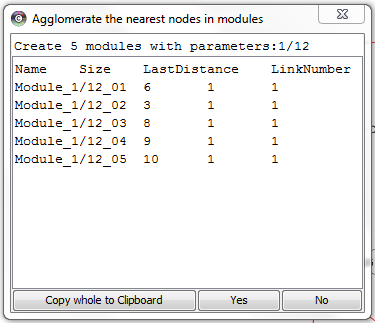
\includegraphics[width=0.8\textwidth]{graphics/Agglomerate_in_modules_dialog}
\caption{This window displays modules, number of node, last distance and number of links of agglomerating process. Yes lauches the process of agglomerating.}
\label{Agglomerate_in_modules_dialog}
\end{figure}
\begin{figure}
\centering
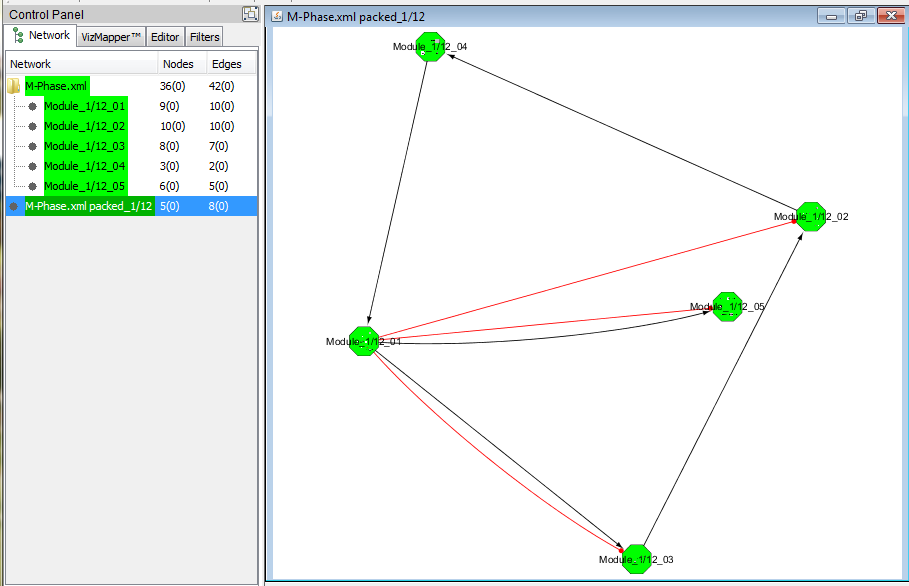
\includegraphics[width=0.8\textwidth]{graphics/M-Phase_packed}
\caption{M-Phase is got by creating network from modules, modules created by agglomerating the nearest nodes (maximal distance=1, maximal size=12 nodes).}
\label{M-Phase_packed}
\end{figure}

\subsection{List Nodes of Modules and Network}
\textbf{Plugins$\Rightarrow$BiNoM 2.1$\Rightarrow$BiNoM Module Manager$\Rightarrow$List Nodes of Modules and Network}\\
List nodes of network and nodes included in modules.\\
Result in text box can be simply copied in a spreadsheet through clipboard.

\subsection{Find Common Nodes in Modules}
\textbf{Plugins$\Rightarrow$BiNoM 2.1$\Rightarrow$BiNoM Module Manager$\Rightarrow$Find Common Nodes in Modules}\\
Display in text box the belonging matrix of nodes (modules in columns, nodes in rows, size of modules in last row, frequency in modules in last column); result more easily usable after copying in a spreadsheet (see~\ref{Common_nodes_in_modules}.\\\\
Create intersection edges with number of common nodes as attribute (COMMON\_NODES), green edges in figure~\ref{M-Phase_Material_Modular}.\\\\
Create node attribute containing the node numbers of modules (NODE\_NUMBER).\\\\
Module Visual StyleCan be adapted to the wished visual aspect by hands in VizMapper, for example:
\begin{itemize}
\item To visualize NODE\_NUMBER: double click Node Size, select NODE\_NUMBER, continuous mapping, adjust width by graphical view.
\item To visualize COMMON\_NODES double click Edge Line Width, select COMMON\_NODES, continuous mapping, adjust width by graphical view.
\end{itemize}
\begin{figure}
\centering
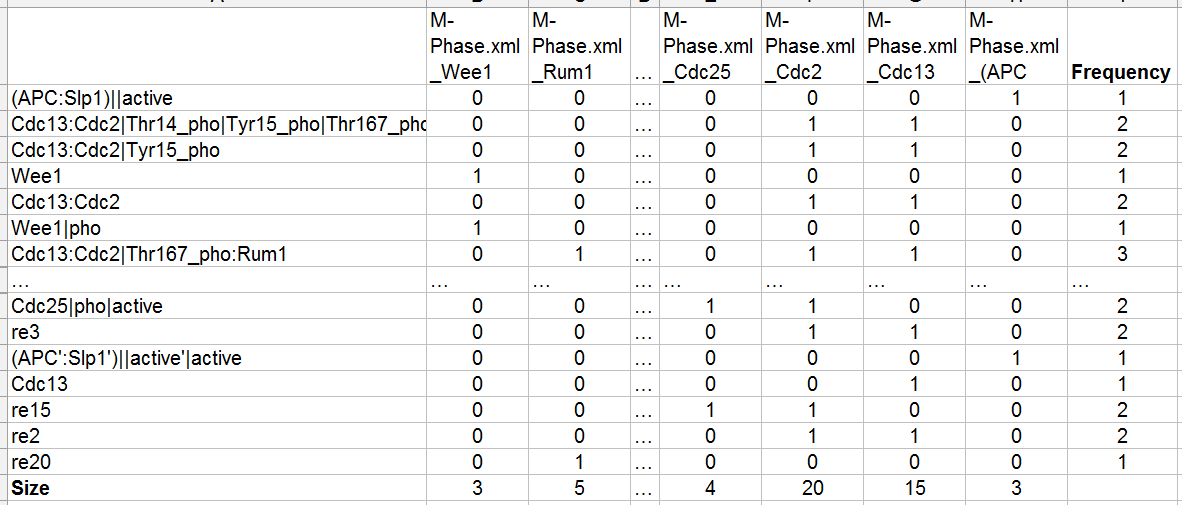
\includegraphics[width=0.8\textwidth]{graphics/Common_nodes_in_modules}
\caption{Matrix of nodes: modules in columns, nodes in rows, size of modules in last row, frequency in modules in last column.}
\label{Common_nodes_in_modules}
\end{figure}

\subsection{Assign Module Names to Node Attribute}
\textbf{Plugins$\Rightarrow$BiNoM 2.1$\Rightarrow$BiNoM Module Manager$\Rightarrow$Assign Module Names to Node Attribute}\\
Create a node attribute (named as the modular network), containing module names. This attribute may be used to visualize modules in the reference network.

\subsection{List Components of Species in Network and Modules}
\textbf{Plugins$\Rightarrow$BiNoM 2.1$\Rightarrow$BiNoM Module Manager$\Rightarrow$List Components of Species in Network and Modules}\\
List components of species (their names must respect BiNoM syntax). Useful to name modules.

\subsection{Create Network from Union of Selected Modules}
\textbf{Plugins$\Rightarrow$BiNoM 2.1$\Rightarrow$BiNoM Module Manager$\Rightarrow$Create Network from Union of Selected Modules}\\
Create a network from union of selected modules and its corresponding module in the current network (named by module names separated by \&).

\subsection{Create Network from Intersection of 2 Selected Modules}
\textbf{Plugins$\Rightarrow$BiNoM 2.1$\Rightarrow$BiNoM Module Manager$\Rightarrow$Create Network from Intersection of 2 Selected Modules}\\
Create a network from intersection of 2 selected modules and its corresponding module (named by module names separated by \textbar.\\\\
Confirm for deleting the common nodes in the selected modules.

\subsection{Recreate Lost Connections inside Modules}
\textbf{Plugins$\Rightarrow$BiNoM 2.1$\Rightarrow$BiNoM Module Manager$\Rightarrow$Recreate Lost Connections Inside Modules}\\
Recreate connections inside modules which may have been lost by modularizing operations.

\subsection{Destroy Networks Unused as Module}
\textbf{Plugins$\Rightarrow$BiNoM 2.1$\Rightarrow$BiNoM module manager$\Rightarrow$Destroy Networks Unused as Module}\\
Select networks to be deleted among a list of networks which are not used as modules in the current network (simplify cleaning session).

\newpage
\section{BiNoM BioPAX3 Utils}
\begin{figure}[h]
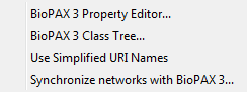
\includegraphics{graphics/BiNoM_BioPAX3_Utils}
\end{figure}
\newpage
\section{BiNoM BioPAX3 Query}
\begin{figure}[h]
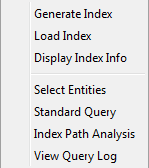
\includegraphics{graphics/BiNoM_BioPAX3_Query}
\end{figure}
\newpage
\section{BiNoM Utilities}
\begin{figure}[h]
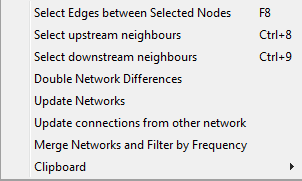
\includegraphics{graphics/BiNoM_Utilities}
\end{figure}
\newpage
 \bibliographystyle{plain}
 \bibliography{BiNoM_Manual}
\end{document}
